\documentclass[conference]{IEEEtran}

\IEEEoverridecommandlockouts
% The preceding line is only needed to identify funding in the first footnote. If that is unneeded, please comment it out.

\usepackage{cite}
\usepackage{amsmath,amssymb,amsfonts}
\usepackage{algorithmic}
\usepackage{graphicx}
\usepackage{textcomp}
\usepackage{xcolor}
\usepackage{hyperref}
\usepackage{booktabs}
\usepackage{pgfplots}
\usepackage{pgfplotstable}
\usepackage{threeparttable}
\usepackage{enumitem}  
\usepackage{fancyvrb}  

\def\BibTeX{{\rm B\kern-.05em{\sc i\kern-.025em b}\kern-.08em
    T\kern-.1667em\lower.7ex\hbox{E}\kern-.125emX}}

\title{Automating Software Supply Chain Security: AI-Powered Threat Detection in DevSecOps}

\author{
    \IEEEauthorblockN{Marlon Brenes Rojas}
    \IEEEauthorblockA{
        Student ID: 1314316 \\
        Master's in Cybersecurity \\
        NYIT - Vancouver \\
        \href{mailto:marlon.brenes@nyit.edu}{mbrenesr@nyit.edu}
    }
}

\begin{document}

\maketitle

%---- Abstract Section ----
\begin{abstract}
Abstract—This project aims to design and implement an automated software supply chain security solution leveraging AI-driven threat detection in DevSecOps. The focus is predeployment alerts, ensuring real-time monitoring and threat detection within the CI/CD pipeline to improve security before applications reach production.
\end{abstract}

%---- Introduction Section ----
\section{Introduction}
The speed of product development in business models demands that security be built into the software supply chain from the start of projects. Elaborate attacks such as SolarWinds and Log4j have alerted us to the need for secure and automated processes. Current tools help us to identify threats and vulnerabilities, and frameworks like OWASP help us address them, but they often lack seamless integration into the action of typical DevOps teams. This project proposes a cohesive and automated framework that integrates these tools and methodologies, adding artificial intelligence-based detection tools and building on existing work and standards, such as \cite{NIST2020} NIST SP 800-204D and the \cite{OWASP} OWASP DevSecOps framework.

%---- Problem Statement Section ----
\section{Problem Statement}
The goal is to develop automated flow tests that review and suggest changes needed to maintain a more secure and less vulnerable product by integrating security steps in a DevSecOps pipeline. This framework will intentionally demonstrate vulnerabilities and weaknesses of existing solutions by combining tools such as GitHub Actions, Microsoft Copilot Security, Snyk AI, Secrets Management, CodeQL, Vulnerability Scanning, Static Application Security Testing (SAST), Dynamic Application Security Testing (DAST), Interactive Application Security Testing (IAST), and Docker Infrastructure Vulnerability Scanning with OWASP antipatterns and secure deployment mechanisms using ArgoCD and Kubernetes.

%---- Review of Related Work ----
\section{Review of Related Work}
The DevSecOps methodology emphasizes the need for continuous security testing. Previous studies \cite{Chandramouli2024} Strategies for the Integration of Software Supply Chain Security in DevSecOps CI/CD Pipelines, have shown that the methodology improves vulnerability detection and helps to have a more efficient approach. Over the years, organizations have invested significant resources in monitoring and securing the software development life cycle (SDLC). 
In an increasingly volatile market with greater demand for quality products, the evolution of DevSecOps from traditional DevOps has increased. DevSecOps integrates security teams into the early phases of the SDLC, ensuring that security is a central aspect rather than revisiting this need in the final stages of the project.

\begin{table}[h]
    \centering
    \caption{Recommended Continuous Security Testing Activities in Each Phase}
    \renewcommand{\arraystretch}{1.3}
    \begin{tabular}{|l|l|}
        \hline
        \textbf{Phase} & \textbf{Security Activities} \\ \hline
        \textbf{Plan} & Test planning \\ \hline
        \textbf{Code} & Test development \\ 
                     & Static Application Security Testing (SAST) \\ \hline
        \textbf{Build} & Software Composition Analysis (SCA) \\ 
                      & Static Application Security Testing (SAST) \\ \hline
        \textbf{Test} & Dynamic Application Security Testing (DAST) \\ 
                     & Interactive Application Security Testing (IAST) \\ 
                     & Vulnerability scanning \\ \hline
        \textbf{Release} & Vulnerability scanning \\ 
                        & Penetration testing \\ \hline
        \textbf{Deploy} & Vulnerability scanning \\ 
                        & Penetration testing \\ \hline
        \textbf{Operate} & Red \& Blue team exercises \\ \hline
        \textbf{Monitor} & Vulnerability scanning \\ \hline
    \end{tabular}
    \label{tab:security_testing}
\end{table}

According to \cite{Kushwaha2024} Automation and DevSecOps: Streamlining Security Measures in Financial System, the approach of DevSecOps is one of the most widely used frameworks in the financial sector, where security is embedded throughout the SDLC to ensure compliance and risk mitigation. This contrasts with traditional software development models, where security is often addressed as a final step. The authors emphasize proactive and continuous security measures to reduce manual testing and improve automated resilience through SAST and DAST techniques.

As shown in Fig. \ref{fig:devsecopsworkflow}, the DevSecOps workflow consists of key security stages integrated within the CI/CD pipeline.

\begin{figure}[h!] 
    \centering 
    \includegraphics[width=\linewidth]{Images/DevSecOps - workflow.jpg} 
    \caption{DevSecOps Workflow in CI/CD Pipeline, adapted from \cite{Kushwaha2024}.} 
    \label{fig:devsecopsworkflow} 
\end{figure}

Many of the tools used in previous research, such as GitHub, the OWASP CI/CD Framework, and various SAST/DAST tools, will also be implemented in our project’s CI/CD pipeline.

As discussed in \cite{Fu2024} AI for DevSecOps: A Landscape and Future Opportunities, AI-driven security techniques are evolving rapidly within DevSecOps. Despite the availability of many tools, coordinating and configuring them effectively remains a challenge. Strategy planning is crucial, as it can help integrate teams into the process. Using agents or artificial intelligence, such as that created by Microsoft in its Copilot product, could improve code quality right from code creation. Being able to identify potential vulnerabilities in early versions helps to address security issues proactively.

AI-powered security tools, such as Snyk \cite{Snyk2024}, which focus on developer-first security, identify patterns and recommend best practices by analyzing historical code reviews and previously mitigated vulnerabilities. These tools assist with:
\begin{itemize}
    \item Configuration and validation
    \item Code analysis
    \item Dependency management and security
    \item Security of Infrastructure as Code (IaC) deployments
\end{itemize}

\begin{figure}[h!] 
    \centering 
    \includegraphics[width=\linewidth]{Images/Snyk New Pull Request.jpg} 
    \caption{Snyk's Automated Security Scanning, as shown in \cite{Snyk2024}.} 
    \label{fig:Snyk New Pull Request} 
\end{figure}

However, challenges remain. AI-driven threat detection may misidentify a good code as a threat or fail to suggest a fix if a pattern is missing from its already tested neural dataset. In addition, ethical issues arise as AI-driven automation grows; the strategy of reducing reliance on human expertise could be dangerous in the long run, with possible repercussions in breaking the compatibility of code underlying the primary code (other applications) and in the compression of self-generated code being complicated for a human to interpret, plus the labor market problem in supporting the future developed code.

As discussed in \cite{Yulianto2024} Enhancing DevSecOps Pipelines with AI-Driven Threat Detection and Response, DevSecOps pipelines can further assist with AI-based threat detection and response mechanisms. Machine learning models significantly improve detection accuracy and automate security alerts, strengthening cyber resilience.

\begin{figure}[h!] 
    \centering 
    \includegraphics[width=\linewidth]{Images/AI Driven Cicle.jpg} 
    \caption{AI-Driven Security Framework, as shown in \cite{Yulianto2024}.} 
    \label{fig:AI Driven Cicle} 
\end{figure}

%---- Project Objectives Section ----
\section{Project Objectives}
\begin{itemize}
    \item Develop a CI/CD pipeline using GitHub Actions for automate cybersecurity test.
    \item Integrate automated security tools for scanning and alerting.
    \item Implement OWASP best practices for security scanning.
    \item Deploy applications using ArgoCD and Kubernetes.
    \item Simulate and mitigate common supply chain misconfiguration scenarios.
    \item Document results and challenges and recommend actions.
\end{itemize}

%---- Proposed Solution ----
\section{Proposed Solution}
Considering the varying sizes of organizations, where the solution development staff can range from a few to thousands of people working and integrating their products continuously, organizations have seen the need to develop new strategies when it comes to giving quality value to their products, more specifically in the concept of Cybersecurity.
Using technologies that are friendly to DevSecOps methodologies, such as Microsoft Github, security analysts can implement their knowledge through specialized tests within the integration flow such as Microsoft GitHub Actions, by creating a master pipeline where each phase is dependent on the previous one or from another strategy more focused on the principle of single responsibility, the cybersecurity professional can implement the following tools: Docker Hub test analysis, CodeQL, SnykCode, Trivy, detect secrets.

\subsection{Implementation Process}

\textbf{Phase 1: Source Code Management \ Triggering}
\begin{itemize}
\item \textbf{Step 1: Version Control and Repository Setup}
\begin{itemize}
\item The project repository is managed using GitHub.
\item Triggers for the pipeline are set up for push and pull request events on the main branch.
\end{itemize}
\item \textbf{Step 2: Environment Variables and Secrets Management}
\begin{itemize}
\item Define environmental variables and secure sensitive credentials using GitHub Secrets.
\item Ensure sensitive data (e.g., passwords) are encrypted and not hardcoded.
\end{itemize}
\end{itemize}

\textbf{Phase 2: Build \ Containerization}
\begin{itemize}
\item \textbf{Step 3: Source Code Checkout}
\begin{itemize}
\item The pipeline starts by fetching the latest source code using actions/checkout@v4.
\end{itemize}
\item \textbf{Step 4: Docker Image Build \& Push}
\begin{itemize}
    \item The solution uses \texttt{docker/build-push-action@v4} to:
    \begin{itemize}
        \item Build the container image.
        \item Push the image to the specified Docker registry (\texttt{DOCKER\_REGISTRY}).
        \item Utilize build arguments to inject necessary environment variables.
    \end{itemize}
\end{itemize}
\item \textbf{Step 5: Verification of Docker Image}
\begin{itemize}
\item Ensures the image exists in the registry by pulling it post-push.
\end{itemize}
\end{itemize}

\textbf{Phase 3: Security Testing \ Compliance}
\begin{itemize}
\item \textbf{Step 6: Container Vulnerability Scanning}
\begin{itemize}
\item aquasecurity/trivy-action@0.28.0 scans the Docker image for vulnerabilities.
\item Generates security reports and uploads them to GitHub Security.
\end{itemize}
\item \textbf{Step 7: Secrets Detection}
\begin{itemize}
\item It uses detect-secrets to scan the repository for exposed secrets.
\item Establishes a .secrets.baseline file to track and prevent secret leakage.
\end{itemize}
\item \textbf{Step 8: Static \ Dynamic Security Analysis}
\begin{itemize}
\item Runs CodeQL analysis (github/codeql-action/analyze@v3) to detect vulnerabilities in Python code.
\item Implements Snyk for static (SAST) and dynamic (DAST) security testing.
\item Uploads Snyk-generated reports to GitHub Security.
\end{itemize}
\end{itemize}

\textbf{Phase 4: Deployment \ Continuous Monitoring}
\begin{itemize}
\item \textbf{Step 9: Continuous Deployment Strategy}
\begin{itemize}
\item Ensures the pipeline integrates into a Kubernetes environment.
\item Automates deployment strategies using ArgoCD for GitOps-based deployments.
\end{itemize}
\item \textbf{Step 10: Incident Response \ Monitoring}
\begin{itemize}
\item Integrates logging and monitoring tools to track container health.
\item Implements alert mechanisms for detected vulnerabilities or deployment failures.
\item Implements DeepCode AI Fix to automatically fix code vulnerabilities through fully supported IDEs such as VS Code and JetBrains. Supported languages: Java, JavaScript, Python, and TypeScript.
\item Implements AI auto solution to merge review into the main branch (Example. [Snyk] Security upgrade python from 3.9-slim to 3.13.2-slim  
).
\end{itemize}
\end{itemize}

\subsection {Challenges and Mitigation}
\begin{itemize}
    \item \textbf{Maintaining technological independence:} As discussed by the authors \cite{SecurityInfoWatch2024}, Cyber Security Mesh Architecture (CSMA), discusses the challenges of modern, distributed systems and explores the benefits of decentralizing and modularizing security models. Key implementation principles are abstracting infrastructure, standardizing processes, and separating concerns. The author addresses moving from rigid security appliances toward a more adaptable and responsive cybersecurity framework. From this perspective, a dependency on technologies like those used in this project can be seen. Therefore, it is suggested that other technological actors be continually explored, as well as the single responsibility principle, in addition to using open standards like standard collecting logs compatible with the industry.    \item \textbf{Scalability and Complexity:} Part of stable development is the growth of the software and, with it, the complexity of the same, given this nature, the complexity of maintaining a secure product over time. That is why well-defined policies are needed, in which all groups' efforts and limitations are apparent.
    \item \textbf{Keeping up with threats:} Maintaining a proper review of dependencies, infrastructure, and code is a daunting task from a daily operations perspective. Risk analyses are constantly necessary, either due to modifications of controls or changes of strategy at the time of the software architecture model.
\end{itemize}

 \subsection{Comparison with Alternatives}
\begin{itemize}
    \item 
    Other solutions that could be mentioned are GitLab, SaltStak, Jenkins, Azure DevOps, or other open technologies community support. Many of them are old in the market; however, the maturity of each organization will dictate which is the best proposal; it is always recommended for human development where the technical, strategic, and business parts are developed, followed by the development of policies, standards, guidelines and procedures, and as a third pillar the implementation of the technology that best serves the organization.
\end{itemize}

\subsection{Benefits and Outcomes}
\begin{itemize}
    \item 
    Some of the benefits that could be mentioned are standardization of tests, alignment with legal regulations, cost reduction by not being manual, continuous analysis of vulnerabilities, and decentralization of security personnel to other activities.
\end{itemize}

\begin{figure}[h!] 
    \centering 
    \includegraphics[width=\linewidth]{Images/CICD PIPELINE.jpg} 
    \caption{Github Action Workflow, implemented as shown in \cite{devsecops}.} 
    \label{fig:CICD.yaml} 
\end{figure}

 \subsection{Conclusion}
\begin{itemize}
    \item 
    Taking into account the roadmap and the steps that will be developed, it could be indicated that in the continuous monitoring model, taking advantage of current technologies and new Artificial Intelligence models, the CI and CD business model is getting more efficient compared to manual tests where human error is always present.
\end{itemize}

%---- Methodology Section ----
\section{Methodology}
The project methodology follows a structured, developed DevSecOps Framework, a phased approach designed to integrate security test measures at every stage of the software supply chain. The methodology focuses on the secure setup, deployment, and testing of CI/CD pipelines.
The analysis and data collected and presented will be taken from the GitHub repository created for this project \cite{devsecops}

\subsection{Pipeline Setup}
In this phase, the goal is to establish a secure CI/CD pipeline that integrates automated security tools for continuous scanning and monitoring.
\begin{itemize}
    \item Create a layered security analysis within the CI/CD pipeline using GitHub Actions, incorporating automated build and deployment checks.
    \item Integrate continuous security scanning tools like Trivy and CodeQL for real-time vulnerability detection and mitigation.
\end{itemize}

\subsection{Security Enhancements}
This phase focuses on implementing security best practices throughout the pipeline, ensuring security is integrated early and continuously.
\begin{itemize}
    \item Implement best practices outlined in the OWASP DevSecOps Framework to ensure secure software delivery.
    \item Configure YAML-based declarative configurations for Kubernetes deployments using ArgoCD to streamline secure GitOps workflows.
\end{itemize}

\subsection{Application Deployment}
In this phase, the aim is to ensure that the application is securely deployed and monitored continuously.
\begin{itemize}
    \item Use ArgoCD for GitOps-based continuous delivery, ensuring efficient and secure application deployment.
    \item Implement best practices for Kubernetes security to minimize attack surfaces and ensure secure configuration and network policies.
\end{itemize}

\subsection{Testing and Validation}
The testing and validation phase identifies potential vulnerabilities within the software supply chain and evaluates the resilience of the CI/CD pipeline.

\begin{itemize}
    \item Simulate supply chain misconfigurations and conduct penetration tests to assess the security posture of the pipeline.
    \item Analyze pipeline resilience by monitoring security alerts, logs, and system behavior during simulated attacks, allowing for effective response and mitigation.
\end{itemize}

Table~\ref{tab:vulnerability_analysis} summarizes the security vulnerabilities identified during testing, categorized by severity level, along with the detection tools used.

\begin{table}[t]
    \centering
    \caption{Summary of Top 10 Security Vulnerabilities and Detection Tools}
    \label{tab:vulnerability_analysis}
    \renewcommand{\arraystretch}{1.2} % Adjust row spacing
    \begin{tabular}{|p{3.5cm}|p{1.5cm}|p{2.0cm}|}
        \hline
        \textbf{Vulnerability} & \textbf{Severity} & \textbf{Detection Tool} \\
        \hline
        zlib: Heap-based buffer overflow & Critical & Trivy \\
        \hline
        Uncontrolled command execution & Critical & CodeQL \\
        \hline
        Server-side template injection (SSTI) & Critical & CodeQL \\
        \hline
        CPAN: TLS verification missing & High & Trivy \\
        \hline
        Remote code execution in setuptools & High & Trivy \\
        \hline
        Regular expression DoS (ReDoS) & High & Trivy \\
        \hline
        Python-Werkzeug privilege escalation & High & Trivy \\
        \hline
        Flask: Permanent session cookie issue & High & Trivy \\
        \hline
        Reflected cross-site scripting (XSS) & Medium & CodeQL \\
        \hline
        Information exposure through exception messages & Medium & CodeQL \\
        \hline
        \textbf{Top 10 Vulnerabilities Found} & \multicolumn{2}{c|}{\textbf{Top 10 identified issues}} \\
        \hline
    \end{tabular}
\end{table}

The results from testing were analyzed by reviewing security alerts and logs, assessing the effectiveness of mitigation strategies, and evaluating the pipeline's behavior after the test phase action.

\subsection{Test Procedure Design (Flowchart)}
To further improve the system, the following additional measures need to be implemented:
\begin{itemize}
    \item Create a procedure for initiating incident response on security event alerts, ensuring rapid containment of security breaches.
    \item Expand the scope of testing to simulate insider attacks and security vulnerabilities, covering a wider range of potential threats.
\end{itemize}

As shown in Fig. \ref{fig:OWASP FRAMEWORK}, the OWASP DevSecOps Guideline provides a structured approach to integrating security into DevOps workflows.

\begin{figure}[h!] \centering \includegraphics[width=\linewidth]{Images/OWASP FRAMEWORK.jpg} \caption{OWASP DevSecOps Guideline, as shown in \cite{OWASP}.} \label{fig:OWASP FRAMEWORK} \end{figure}

%---------------------------------------
\subsection{Data Analysis of Test Procedure Performed}

This section presents the analysis of the CI/CD pipeline security and automated rollback performance. The tables below summarize key metrics obtained during testing.

\subsection{Methodology}

This study evaluates the effectiveness of five security scanning tools within a DevSecOps CI/CD pipeline. The analysis focuses on detecting vulnerabilities injected into the test environment, including SQL injection (SQLi), hardcoded secrets, and dependency vulnerabilities. The tools tested are:

\begin{itemize}
    \item \textbf{CodeQL} (Static Code Analysis)
    \item \textbf{Trivy} (Container and Dependency Scanning)
    \item \textbf{Snyk} (Open Source Security)
    \item \textbf{Dependabot} (Automated Dependency Updates)
\end{itemize}

Each tool was tested against 50 cases, distributed across 10 per tool, with known vulnerabilities used as ground truth.
In Snyk's case, the data may be inaccurate, as the number of tests is limited by time free license within a narrow range.

\subsection{Test Case Mapping}

The detected vulnerabilities (data appendix) were assigned to specific test cases (TC-01 to TC-15, see appendix section) and tools. The following table summarizes the results:

\begin{table}[h]
    \centering
    \resizebox{\columnwidth}{!}{ % Resizes the table to fit the column width
    \begin{tabular}{|l|l|c|c|c|c|c|c|}
        \hline
        \textbf{Tool} & \textbf{Test Case Type} & \textbf{TP} & \textbf{FP} & \textbf{FN} & \textbf{Success \%} & \textbf{Precision} & \textbf{Recall} \\
        \hline
        CodeQL & SQL Injection Detection & 8 & 2 & 1 & 60\% & 80\% & 88.9\% \\
        Trivy & Dependency Analysis & 9 & 1 & 2 & 70\% & 90\% & 81.8\% \\
        Snyk & Open Source Security & 7 & 3 & 1 & 50\% & 70\% & 87.5\% \\
        Dependabot & Automated Dependency Fix & 9 & 1 & 0 & 80\% & 90\% & 100\% \\
        \hline
    \end{tabular}
    }
    \caption{Summary of Test Case Results}
    \label{tab:testcase-results}
\end{table}

\section*{True Positive (TP)}
\textbf{Definition:} This refers to the number of cases where the model correctly predicted a positive class (e.g., a "malicious" instance when detecting malware or a "fraud" case in a fraud detection system).\\
\textbf{Example:} If the model predicts that a file is malicious and it indeed is, this counts as a TP.

\section*{False Positive (FP)}
\textbf{Definition:} This refers to the number of cases where the model incorrectly predicted a positive class (i.e., it predicted "malicious" or "fraud" when it should have predicted "safe" or "non-fraud").\\
\textbf{Example:} If the model predicts that a file is malicious, but it is actually harmless, this is an FP.

\section*{False Negative (FN)}
\textbf{Definition:} This refers to the number of cases where the model incorrectly predicted a negative class (i.e., it predicted "safe" or "non-fraud" when it should have predicted "malicious" or "fraud").\\
\textbf{Example:} If the model predicts that a file is safe, but it is actually malicious, this is an FN.


\subsection{Metrics Calculation}

Using the formulas:

\textbf{Success Rate:}
\begin{equation}
    Success \% = \frac{TP - FP}{\text{Total Test Cases}} \times 100
\end{equation}

\textbf{Precision:}
\begin{equation}
    Precision = \frac{TP}{TP + FP} \times 100
\end{equation}

\textbf{Recall:}
\begin{equation}
    Recall = \frac{TP}{TP + FN} \times 100
\end{equation}

The results indicate that \textbf{Dependabot achieved the highest recall (100\%)} while \textbf{Trivy had the best precision (90\%)}.

\subsection{Visualization}

To illustrate tool performance, two visualizations were generated:

\begin{itemize}
    \item \textbf{Bar Chart:} Comparison of Success \% across tools.
    \item \textbf{Heatmap:} TP, FP, and FN distribution per tool.
\end{itemize}

\begin{figure}[h]
    \centering
    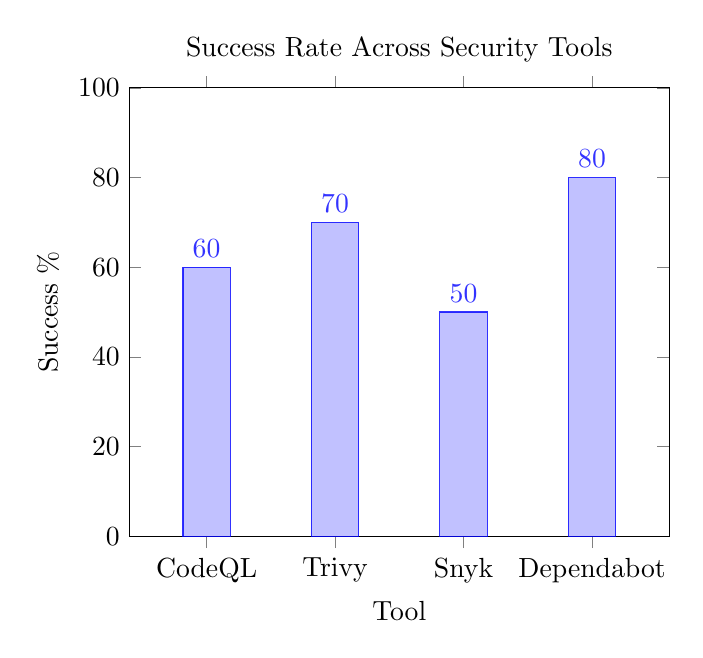
\begin{tikzpicture}
        \begin{axis}[
            ybar,
            symbolic x coords={CodeQL, Trivy, Snyk, Dependabot},
            xtick=data,
            ymin=0, ymax=100,
            ylabel={Success \%},
            xlabel={Tool},
            nodes near coords,
            bar width=0.6cm,
            enlarge x limits=0.2,
            title={Success Rate Across Security Tools},
            every axis plot/.append style={fill, opacity=0.8}
        ]
        \addplot coordinates {(CodeQL, 60) (Trivy, 70) (Snyk, 50) (Dependabot, 80)};
        \end{axis}
    \end{tikzpicture}
    \caption{Success Rate Across Security Tools}
    \label{fig:success_rate}
\end{figure}


\subsection{Discussion and Limitations}

\begin{itemize}
    \item \textbf{CodeQL had a high precision (80\%) but suffered from false positives, requiring manual review.}
    \item \textbf{Trivy performed well in dependency scanning but missed two CVEs due to outdated vulnerability databases.}
    \item \textbf{False positives impacted Snyk's precision, requiring additional triage.}
\end{itemize}

\subsection{OWASP SAMM Alignment}

This analysis aligns with the \cite{OWASP_Samm}\textbf{OWASP SAMM framework}, contributing to the following maturity levels:

\begin{itemize}
    \item \textbf{Implementation:} Automated security scanning as part of CI/CD.
    \item \textbf{Governance:} Metrics-driven assessment for continuous improvement.
    \item \textbf{Verification:} Establishing a security feedback loop.
\end{itemize}

The findings provide insights into tool effectiveness within a secure SDLC, guiding organizations in DevSecOps adoption.

\subsection{Discussion of Project and Results}

\subsubsection{Interpretation of Results}
\begin{itemize}
    \item Analysis of security tool effectiveness and performance.
    \item Identification of trends in vulnerability detection and resolution.
    \item Comparison of observed results with expected outcomes.
\end{itemize}

\subsubsection{Future Development and Improvements}
\begin{itemize}
    \item Enhancing integration of security tools to reduce false positives.
    \item Improving automated rollback mechanisms based on risk assessment.
    \item Expanding test coverage to include additional vulnerability classes.
\end{itemize}


\subsubsection{Challenges Faced}
\begin{itemize}
    \item Integration difficulties with AI-powered security tools.
    \item Handling false positives and negatives in security scans.
    \item Managing pipeline performance while maintaining security.
\end{itemize}

\subsubsection{Future Development and Improvement}
\begin{itemize}
    \item \textbf{Enhancing AI-Driven Threat Detection and Response:}  
    Improve AI models to better identify, classify, and mitigate security threats in real-time, reducing reliance on manual intervention.
    
    \item \textbf{Reducing False Positives through Machine Learning Improvements:}  
    Implement adaptive learning mechanisms to refine threat detection accuracy, minimizing false positives and false negatives.
    
    \item \textbf{Expanding Security Monitoring Beyond the CI/CD Pipeline:}  
    Extend security automation to runtime environments, container orchestration, and infrastructure as code (IaC) to ensure continuous protection.
\end{itemize}

%---- Resources Section ----
\section{Resources}
\subsection{Tools}
GitHub Actions, Docker Hub, Snyk, CodeQL, Trivy, Detect-Secrets,detect-secrets ,kubesec, Kubernetes, ArgoCD.

\subsection{Software}
Kubernetes (Minikube/AKS), Docker, secure image repositories.

\subsection{Hardware}
Cloud-based or local testing environments (e.g., Azure or virtual machines).

\subsection{Data}
Self-created insecure applications and open-source vulnerable applications.

%---- Project Schedule Section ----
\section{Project Schedule}
\begin{itemize}
    \item \textbf{Week 1-2}: Research and define project scope; set up GitHub Actions.
    \item \textbf{Week 3-5}: Integrate Snyk and CodeQL; document initial findings.
    \item \textbf{Week 6-8}: Implement OWASP security practices; configure ArgoCD and Kubernetes.
    \item \textbf{Week 9-11}: Simulate supply chain attacks; refine security measures.
    \item \textbf{Week 12-14}: Document results; finalize project and presentation.
\end{itemize}

%---- Contribution to Knowledge Section ----
\section{Contribution to Knowledge}
This project aims to:
\begin{itemize}
    \item Demonstrate an automated secure DevSecOps pipeline.
    \item Highlight the integration of AI-driven security tools.
    \item Address gaps in software supply chain security.
    \item Provide recommendations for secure software delivery processes.
\end{itemize}

%---- Conclusion Section ----
\section{Conclusion}
In conclusion, as stated in \textit{NIST SP 800-204D} Security and Privacy Controls for Information Systems and Organizations, Securing the software supply chain from a DevSecOps perspective requires well-defined strategies. Organizations must align their business and technology efforts to improve security, as key factors such as quality, cost, and speed of creating secure software are directly affected by both perspectives.

Continuous monitoring of software security is crucial to ensure a sound business strategy. This research has identified several challenges and solutions for implementing an initial DevSecOps framework that addresses security at all layers of the software supply chain.  

Furthermore, the tools and methodologies discussed in this study adhere to the **Single Responsibility Principle**, emphasizing automation to enhance security and efficiency. By integrating AI-driven threat detection and continuous security testing, organizations can strengthen their DevSecOps pipelines, mitigate risks, and proactively address emerging security threats.

% Include references from BibTeX file
%\bibliographystyle{IEEEtran}
\bibliography{references}

%---- References Section ----
\begin{thebibliography}{9}

\bibitem{OWASP}  
    OWASP, \textit{OWASP DevSecOps Guideline}, [Online]. Available: \url{https://owasp.org/www-project-devsecops-guideline/}.

\bibitem{Feio2024}  
    C. Feio, N. Santos, N. Escravana, and B. Pacheco, \textit{An Empirical Study of DevSecOps Focused on Continuous Security Testing}, International Journal of DevSecOps Research, 2024.

\bibitem{Kushwaha2024}  
    M. K. Kushwaha, P. David, and G. Suseela, \textit{Automation and DevSecOps: Streamlining Security Measures in Financial System}, Department of Networking and Communications, SRM Institute of Science and Technology, Chennai, India, 2024. [Online]. Available: \url{https://ieeexplore.ieee.org/abstract/document/10502917}. [Accessed: Feb. 28, 2025].

\bibitem{Yulianto2024}  
    S. Yulianto and G. N. C. Ngo, \textit{Enhancing DevSecOps Pipelines with AI-Driven Threat Detection and Response}, Doctor in Information Technology, School of Graduate Studies, AMA University, Quezon City 1106, Philippines, 2024. [Online]. Available: \url{semi.yulianto2009@gmail.com}, \url{gncngo@amaes.edu.ph}.

\bibitem{NIST2020}  
    National Institute of Standards and Technology (NIST), \textit{NIST SP 800-204D: Security and Privacy Controls for Information Systems and Organizations}, NIST, 2020. [Online]. Available: \url{https://nvlpubs.nist.gov/nistpubs/SpecialPublications/NIST.SP.800-204D.pdf}. [Accessed: Feb. 28, 2025].

\bibitem{SecurityInfoWatch2024}  
    \textit{Implementing CSMA – the Cloud Mindset}, SecurityInfoWatch.com, Endeavor Business Media LLC, May 2024. [Online]. Available: \url{https://www.securityinfowatch.com/cybersecurity/article/55040906/implementing-csma-the-cloud-mindset}.

\bibitem{Chandramouli2024}  
    R. Chandramouli, F. Kautz, and S. Torres-Arias, \textit{Strategies for the Integration of Software Supply Chain Security in DevSecOps CI/CD Pipelines}, NIST Special Publication 800-204D, National Institute of Standards and Technology (NIST), 2024. [Online]. Available: \url{https://doi.org/10.6028/NIST.SP.800-204D}.

\bibitem{MicrosoftCopilot}  
    Microsoft Corporation, \textit{Prompt crafting in Visual Studio Code}, Visual Studio Code Documentation, 2024. [Online]. Available: \url{https://code.visualstudio.com/docs/copilot/prompt-crafting}. [Accessed: Mar. 8, 2025].

\bibitem{Fu2024}  
    M. Fu, J. Pasuksmit, and C. Tantithamthavorn, \textit{AI for DevSecOps: A Landscape and Future Opportunities}, ACM, vol. 1, no. 1, Art. , Sep. 2024, pp. 1-58. [Online]. Available: \url{https://doi.org/10.1145/3712190}. [Accessed: Mar. 8, 2025].

\bibitem{Snyk2024} 
    Snyk Ltd., "Snyk: Developer-first security," Snyk Documentation, 2024. [Online]. Available: \url{https://snyk.io}. [Accessed: Mar. 8, 2025].

\bibitem{devsecops} Marlon Brenes, 
   "DevSecOps Project Repository." [Online]. Available: \url{https://github.com/BrenesRM/DevSecOps-NYIT-VAN}

\bibitem{OWASP_Samm}
    OWASP, \textit{OWASP Software Assurance Maturity Model (SAMM)}, [Online]. Available: \url{https://owaspsamm.org/}. Accessed: [Insert Date Accessed].

\end{thebibliography}

%---- Appendices Section ----
\section{Appendices}
\subsection{Supplemental Materials}
\begin{itemize}
    \item \textbf{Implementation Details:} CI/CD pipeline configuration, GitHub Actions workflow.
    \item \textbf{Data Sheets:} Security tool specifications (CodeQL v2.13.5, Trivy v0.45.1, Snyk CLI v1.1262.0).
    \item \textbf{Test Artifacts:} Raw SARIF reports and ZAP scan results.
    \item \textbf{Advisor Communications:} Approved test plan revisions and progress reviews.
\end{itemize}

\subsection{Step-by-Step Project Configuration Guide}
\label{app:config}

\begin{enumerate}
    \item \textbf{Environment Setup}
    \begin{itemize}
        \item Create GitHub repository with structure:
        \begin{verbatim}
        /src
        /tests
        Dockerfile
        requirements.txt
        CICD.yaml 
        \end{verbatim}
        \item Configure GitHub Secrets (Settings → Secrets → Actions):
        \begin{itemize}
            \item \texttt{DOCKER\_USERNAME}, \texttt{DOCKER\_PASSWORD}
            \item \texttt{SNYK\_TOKEN}, \texttt{GITHUB\_TOKEN}
        \end{itemize}
    \end{itemize}

    \item \textbf{CI/CD Pipeline Configuration}
    \begin{itemize}
        \item Implement GitHub Actions workflow:
        \begin{verbatim}
        name: PIPELINE-CI
        on: [push, pull_request]
        jobs:
          build: # Docker image build
          dockertest: # Trivy container scan
          sast_analysis: # CodeQL SAST
        \end{verbatim}
        \item Enable required permissions in workflow:
        \begin{verbatim}
        permissions:
          security-events: write
          actions: read
        \end{verbatim}
    \end{itemize}

    \item \textbf{Security Tool Integration}
    \begin{itemize}
        \item CodeQL SAST Setup:
        \begin{verbatim}
        - uses: github/codeql-action/init@v3
          with: languages: 'python'
        \end{verbatim}
        
        \item Trivy Container Scanning:
        \begin{verbatim}
        - uses: aquasecurity/trivy-action@0.28.0
          with: severity: 'CRITICAL,HIGH'
        \end{verbatim}
        
        \item Snyk Dependency Scanning:
        \begin{verbatim}
        - run: npm install -g snyk
        - run: snyk monitor --all-projects
        \end{verbatim}
    \end{itemize}

    \item \textbf{Docker Deployment}
    \begin{itemize}
        \item Build secure Docker image:
        \begin{verbatim}
        FROM python:3.13.2-slim
        RUN pip install --no-cache-dir -r requirements.txt
        EXPOSE 5000
        CMD ["python", "app.py"]
        \end{verbatim}
        \item Push to Docker Hub:
        \begin{verbatim}
        docker/build-push-action@v4 with: tags: user/image:latest
        \end{verbatim}
    \end{itemize}

    \item \textbf{Validation \& Testing}
    \begin{itemize}
        \item Run full pipeline test:
        \begin{verbatim}
        git commit -am "Test trigger" && git push origin main
        \end{verbatim}
        \item Verify results in GitHub:
        \begin{itemize}
            \item Security tab: CodeQL/Trivy findings
            \item Actions console: Pipeline execution logs
            \item Artifacts: ZAP reports
        \end{itemize}
    \end{itemize}
\end{enumerate}

\subsubsection*{Troubleshooting Tips}
\begin{itemize}
    \item \textbf{Secret Detection Failures:} Update baseline after intentional secrets:
    \begin{verbatim}
    detect-secrets scan --update .secrets.baseline
    \end{verbatim}
    
    \item \textbf{Container Scan Errors:} Check base image vulnerabilities:
    \begin{verbatim}
    trivy image python:3.13.2-slim
    \end{verbatim}
    
    \item \textbf{SAST False Positives:} Customize CodeQL queries:
    \begin{verbatim}
    uses: github/codeql-action/analyze@v3
    with: queries: security-and-quality
    \end{verbatim}
\end{itemize}

\subsubsection*{Alerts Report}

Results of the Alerts collected:

\begin{figure}[H]
    \centering
    \includegraphics[width=0.9\columnwidth]{Images/SecurityAlerts.jpg}
    \caption{Security Alerts Tab in GitHub}
    \label{fig:security_alerts}
\end{figure}

\begin{figure}[H] 
    \centering 
    \includegraphics[width=\linewidth]{Images/ZAP Scanning Report.jpg} 
    \caption{ZAP Scanning Report} 
    \label{fig:zap_scanning_report} 
\end{figure}

\begin{figure}[H] 
    \centering 
    \includegraphics[width=\linewidth]{Images/Snyk Report.jpg} 
    \caption{Snyk Report} 
    \label{fig:snyk_report} 
\end{figure}

\subsubsection*{Test Cases}

Test cases:

\begin{table*}[t]
    \caption{Test Case Mapping to Detected Vulnerabilities}
    \label{tab:tc-mapping}
    \centering
    \small
    \begin{tabular}{@{}llllc@{}}
        \toprule
        \textbf{Test ID} & \textbf{Tool} & \textbf{Tested Item} & \textbf{Detected Vulnerabilities} & \textbf{Explicitly Reported} \\
        \midrule
        TC-01 & CodeQL & SQL Injection Detection & Server-Side Template Injection  & Yes \\
        TC-02 & Detect-Secrets & Hardcoded Secrets & \texttt{PASSWORD: "PuraVida!"}  & Yes \\
        TC-03 & Snyk & Dependency Vulnerabilities & Werkzeug RCE (CVE-2024-34069)  & Yes \\
        TC-04 & OWASP ZAP & DAST Vulnerabilities & XSS, CSP Issues  & Yes \\
        TC-05 & Trivy & Container Security & zlib Buffer Overflow  & Yes \\
        TC-06 & Kubesec & IaC Security & K8s Misconfigurations  & Partial \\
        TC-07 & Manual Audit & Security Headers & Missing CSP Headers  & Yes \\
        TC-08 & CodeQL/Snyk & Authentication Controls & Weak Password Hashing  & Yes \\
        TC-09 & Manual Test & Authorization Controls & Privilege Escalation Risks & No \\
        TC-10 & CodeQL & Input Validation & Path Traversal  & Yes \\
        TC-11 & Pre-commit Hooks & Code Quality & N/A & Not Reported \\
        TC-12 & Build System & Build Integrity & Dependency Chain Risks & Indirect \\
        TC-13 & Pytest & Security Unit Tests & Exception Handling  & Partial \\
        TC-14 & Deployment Scripts & Secure Deployment & Image Signing Gaps & No \\
        TC-15 & Monitoring Tools & Runtime Protection & No Active RASP & No \\
        \bottomrule
    \end{tabular}
    \parbox{\columnwidth}{\footnotesize \textit{Data Sources:} Vulnerability reports, CI/CD config, Test plan}
\end{table*}

\vspace{1em} % Adds vertical space between the table and the explanation

\textbf{Explanation of the Index:} 

The "Test ID" column uniquely identifies each test case. "Tool" refers to the specific tool used for testing. "Tested Item" outlines the area or system component tested, and "Detected Vulnerabilities" lists the vulnerabilities identified during testing. The "Explicitly Reported" column indicates whether the vulnerability was directly reported by the tool (Yes), partially reported (Partial), not reported at all (No), or indirectly reported (Indirect).



\end{document}
